%--------------------------------------------------------------------------------------
% Este arquivo contém a sua metodologia
%--------------------------------------------------------------------------------------
\chapter{Metodologia} \label{ch:MM} %Uma label é como você referencia uma seção no texto com a tag \ref{}

O Sistema Computacional proposto conta com cinco componentes, dados por um \textit{switch}, roteador, servidor \textit{Web}, servidor de aplicação e servidor de banco de dados, como mostrado na Figura \ref{img:modelo}.

\begin{figure}[H]
    \centering
        \caption{\label{img:modelo} Sistema computacional escolhido.}
        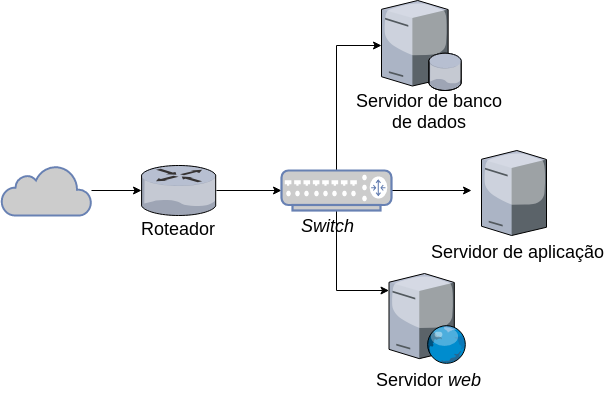
\includegraphics[scale=0.5]{img/modelo.png}
        \legend{\textbf{Fonte: } (Autor, 2019).}
    \end{figure}

Considerando 3000000 pacotes diários, o intervalo entre chegadas foi dado por:

\begin{equation*}
    iat = {\frac{3000000}{24*60*60}}^{-1} = 0,0288 s
\end{equation*}

Por outro lado, os tempos de serviço para cada nível de cada componente são mostrados na Tabela \ref{tbl:componentes}, considerando um pacote de tamanho 5,6 kB.

\begin{table}[!htb]
    \centering
    \caption{\label{tbl:componentes} Descrição dos componentes utilizados.}
        \begin{tabular}{ccm{2.2cm}m{1.9cm}m{2.9cm}m{2.5cm}m{1.6cm}}
            \hline
            \multicolumn{2}{c}{Nível/Fator} & Roteador (A) & \textit{Switch (B)} & Servidor de banco de dados (C) & Servidor de aplicação (D) & Servidor \textit{web} (E) \\ \hline
            \multirow{2}{*}{-1} & Modelo & Model 4451 & SF300-08P & Cassandra & Node.js 10.0.0 & Apache \\
            & $st$ ($10^{-5}$ s/tarefa) & $0,534$ & $0,333$ & $1146,8$ & $1,44$ & $71$ \\ \hline 
            \multirow{2}{*}{+1} & Modelo & Model 4461 & SF300-24P & MongoDB & Node.js 8.0.0 & Nginx \\
            & $st$ ($10^{-5}$ s/tarefa) & $0,356$ & $0,0417$ & $5730$ & $2,02$ & $8,3$ \\ \hline 
        \end{tabular}
    \end{table}
    \legend{\textbf{Fonte: } (Autor, 2019).}

A sequência na qual as tarefas percorrem os componentes foi dada por:

\begin{center}
$S$ = [0, 1, 2, 1, 3, 1, 4, 1, 3, 1, 2, 1, 0]
\end{center}

Em que 0, 1, 2, 3 e 4 correspondem ao roteador, \textit{switch}, servidor \textit{web}, servidor de aplicação e servidor de banco de dados. Por fim, os demais parâmetros da QSN-RI são mostrados na Tabela a seguir.

\begin{table}[!htb]
    \centering
    \caption{Parâmetros da QSN-RI.}
        \begin{tabular}{cc}
            \hline
            Parâmetro & Valor \\ \hline
            N & 1000 \\
            R & 10 \\
            Ni & 0,9*N \\
            qs & 5 \\
            s & 13 \\ \hline
        \end{tabular}
    \end{table}
    \legend{\textbf{Fonte: } (Autor, 2019).}

% \section{Seção de exemplo 1}

As simulações QSN-RI foram conduzidas de acordo com o \textit{script} anexado. Ele foi obtido a partir de Leal (2016) e modificado para a execução dos $2^5$ experimentos, com os resultados sendo salvos em arquivos .csv.



% \subsection{Subseção de exemplo 1 - Referenciando seções} \label{subsec:subsec1}






%--------------------------------------------------------------------------------------
% Insere a seção de cronograma
% Está comentada porque só é necessária no TCC I
%--------------------------------------------------------------------------------------

%\section{Cronograma} \label{sec:crono}

%A tabela \ref{tab:cronograma} mostra o cronograma de atividades a serem executadas para o TCC II, com base no calendário de 201X.Y da UNIVASF.

%\newpage
%\begin{table}[!thb]
%	%\huge
%    \centering
%    \caption{\label{tab:cronograma} Cronograma das atividades previstas para o TCC II}
%%    \begin{adjustbox}{max width=\textwidth}
%    \begin{tabular}{p{6.5cm}|c|c|c|c|c|c}
%    \toprule
%    \textbf{Atividade}                      & Nov & Dez & Jan & Fev & Mar & Abr \\ \hline
%    Implementar o banco de dados              & X    & X     &       &        &          &          \\ \hline
%    Desenvolver a API HTTP RESTful                      &   X   & X     &       &        &          &          \\ \hline
%    Implementar o serviço de captura de dados        &      &      & X     &   X     &          &          \\ \hline
%    Desenvolver a aplicação \textit{Web/mobile} para exibição dos dados         &      &      & X     &   X     &     X     &          \\ \hline
 %   Teste do sistema            &      &       &       &        & X        &          %\\ \hline
 %   Escrita do TCC II                       &   X   & X     & X     & X      & X        & X        \\ \hline
%   Defesa do TCC II                        &      &       &       &        &          & X       \\
%    \bottomrule
 %   \end{tabular}
 %   \end{adjustbox}
%    \legend{\textbf{Fonte:} O autor.}
%\end{table}

